The photon sample used to estimate the $Z$+jets background has contributions from physics processes other than $\gamma$+jets.
Such processes include $Z+\gamma$ events where the $Z$ boson decays into neutrinos. The MET from such events does not come from
jet mismeasurement and as a consequence will bias the $Z$+jets estimate. This section describes our investigation of the 
contamination in the $\gamma$+jets sample.

Our approach to estimate this contamination is to rely on Monte Carlo for processes with real MET; to first order, the missing
energy from such processes are adequately modelled by the simulation. To mimic conditions in data taking, pile-up re-weighting
is applied to the Monte Carlo as well as correction factors to account for the effective luminosity collected from prescaled
photon triggers. 

\subsection{Monte Carlo Samples}

The Monte Carlo samples used in this study are listed in Table~\ref{tab:DatasetsMCPhoJets}. The cross sections for the $W(\ell\nu)+\gamma$ 
and $Z(\ell\ell)+\gamma$ samples include NLO $k$-factors.

\begin{table}[!ht]
\begin{center}
{\footnotesize
\begin{tabular}{|c|l|c|}
\hline
\multicolumn{3}{|c|}{With Pileup: Processed dataset name is always} \\
\multicolumn{3}{|c|}{Summer11-PU\_S4\_START42\_V11-v*/AODSIM} \\
\hline
 Dataset Description                     &   Primary Dataset Name   & cross-section (pb)\\
\hline
$W(e\nu)+\gamma$                    &	/WGToENuG\_TuneZ2\_7TeV-madgraph		  &  137.3 \\
$W(\mu\nu)+\gamma$                  &	/WGToMuNuG\_TuneZ2\_7TeV-madgraph		  &  137.3 \\
$W(\tau\nu)+\gamma$                 &	/WGToTauNuG\_TuneZ2\_7TeV-madgraph-tauola	  &  137.3 \\
$W\rightarrow\ell\nu$               &	/WJetsToLNu\_TuneZ2\_7TeV-madgraph-tauola	  &  31314.0 \\
$Z(ee)+\gamma$                      &	/ZGToEEG\_TuneZ2\_7TeV-madgraph 		  &  42.7 \\
$Z(\mu\mu)+\gamma$                  &	/ZGToMuMuG\_TuneZ2\_7TeV-madgraph		  &  41.975 \\
$Z(\tau\tau)+\gamma$                &	/ZGToTauTauG\_TuneZ2\_7TeV-madgraph-tauola	  &  38.4375 \\
$Z$[50-inf] $\rightarrow\ell\ell$   &	/DYJetsToLL\_TuneZ2\_M-50\_7TeV-madgraph-tauola   &  3048.0 \\
$Z(\nu\nu)+\gamma$                  &	/ZGToNuNuG\_TuneZ2\_7TeV-madgraph		  &  3.426 \\
$\gamma\gamma$[10-25] (Born)        &	/DiPhotonBorn\_Pt-10To25\_7TeV-pythia6  	  &  236.4 \\
$\gamma\gamma$[25-250] (Born)       &	/DiPhotonBorn\_Pt-25To250\_7TeV-pythia6 	  &  22.37 \\
$\gamma\gamma$[250-inf] (Born)      &	/DiPhotonBorn\_Pt-250\_7TeV-pythia6		  &  0.008072 \\
$\gamma\gamma$[10-25] (box)         &	/DiPhotonBox\_Pt-10To25\_7TeV-pythia6		  &  358.2 \\
$\gamma\gamma$[25-250] (box)        &	/DiPhotonBox\_Pt-25To250\_7TeV-pythia6  	  &  11.37 \\
$\gamma\gamma$[250-inf] (box)       &	/DiPhotonBox\_Pt-250\_7TeV-pythia6		  &  0.000208 \\
\hline
\end{tabular}
}
\caption{Summary of Monte Carlo datasets used.}
\label{tab:DatasetsMCPhoJets}
\end{center}
\end{table}

\subsubsection{$W$+jets vs. $W+\gamma$}
The effects of ISR and FSR photon radiation are simulated in both the $W$+jets and $W+\gamma$ Monte Carlo samples. To avoid double
counting, such processes are filtered from the $W$+jets sample by checking the generator level information.

The properties of the events which contribute to the $\gamma+$jets contamination are quite different between $W$+jets and $W+\gamma$
events. For events with a selected photon with $p_T>55\:\GeVc$ and MET $>50\:\GeV$, the $\eta$ distribution of the generated lepton 
and $\Delta R$ between the generated lepton and the photon are shown in Fig.~\ref{fig:CompareWMC1}. It's clear from the $\eta$ plots
that the contribution from $W$ processes is not primarily due to the lepton going out of acceptance, since most of the generated leptons
fall within $|\eta|<2.5$. This suggests that it is the inefficiency of the lepton reconstruction or selection cuts that allow such 
events to be included in the $\gamma+$jets control sample. The $\Delta R$ distribution for $W+$jets indicates the reconstructed photon 
object is likely a mis-identified electron. This hypothesis is further supported when breaking down the $\Delta R$ distribution into 
the different lepton decay modes in Fig.~\ref{fig:CompareWMC2}. For $W+$jets, the electron decay mode is the dominant contribution.

%%%%%%%%
\begin{figure}[!hbtp]
\begin{center}
\subfigure[Inclusive]{\label{subfig:eta}
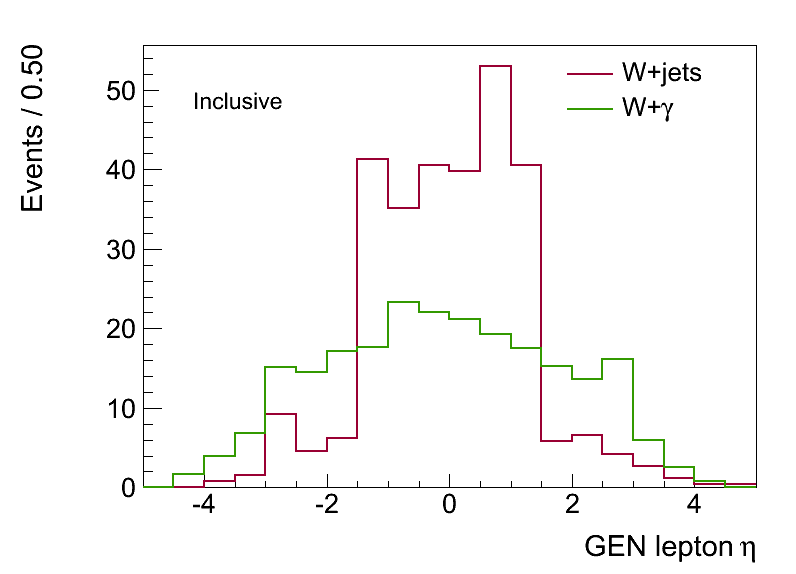
\includegraphics[width=.4\textwidth]{figures/eta_incl.png}}
\subfigure[0-Jet]{\label{subfig:dr}
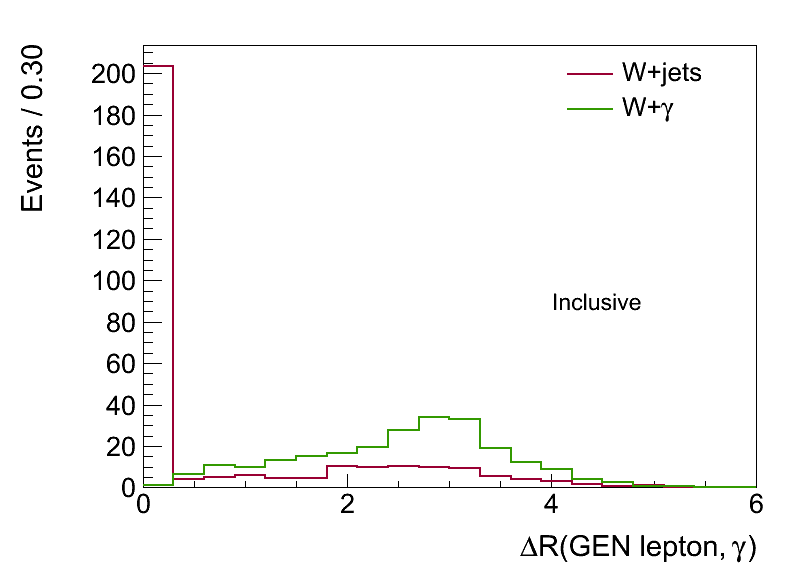
\includegraphics[width=.4\textwidth]{figures/dr_incl.png}}
\caption{\subref{subfig:eta} $\eta$ of the generated lepton from $W$ decay. \subref{subfig:dr} $\Delta R$ between
the generated lepton and the selected photon. Events are selected with photon $p_T>55\:\GeV/c$ and MET $>55\:\GeV$. Each
MC sample is scaled to $1\:\ifb$.}
\label{fig:CompareWMC1}
\end{center}
\end{figure}
%%%%%%%%

%%%%%%%%
\begin{figure}[!hbtp]
\begin{center}
\subfigure[Inclusive]{\label{subfig:dr_wjets}
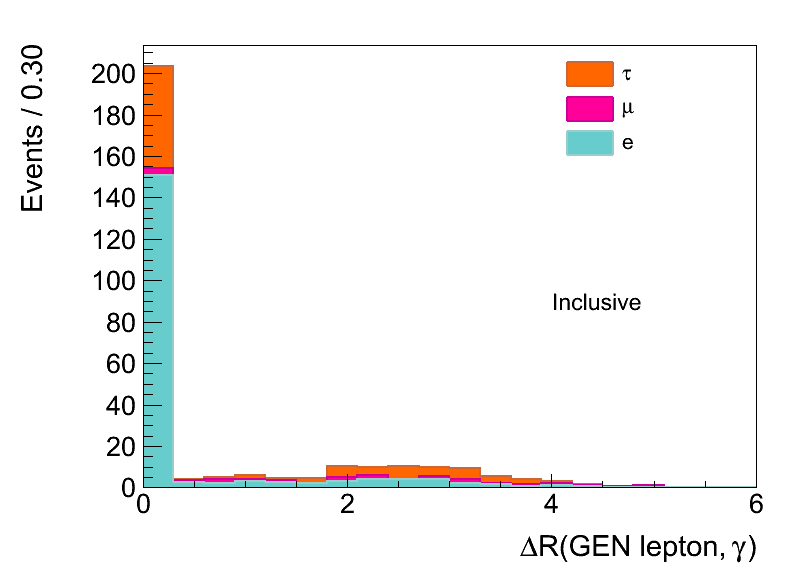
\includegraphics[width=.4\textwidth]{figures/dr_wjets_incl.png}}
\subfigure[0-Jet]{\label{subfig:dr_wgamma}
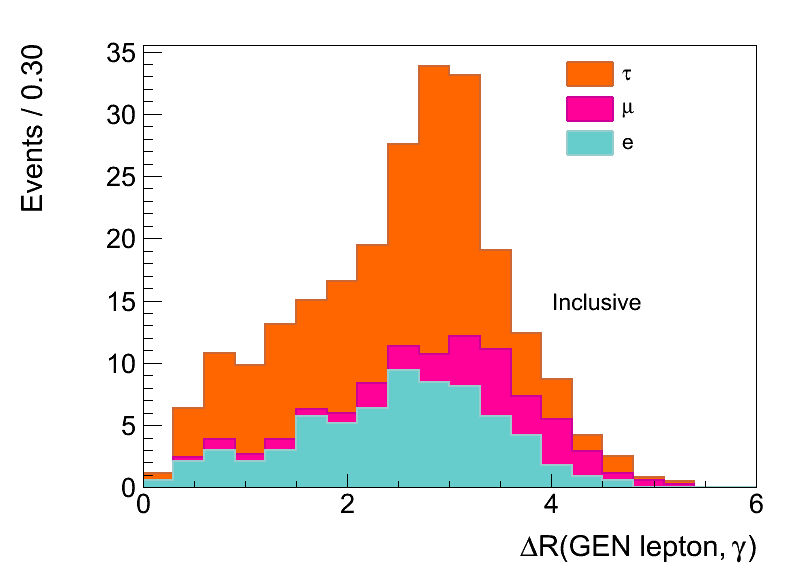
\includegraphics[width=.4\textwidth]{figures/dr_wgamma_incl.png}}
\caption{$\Delta R$ between the generated lepton and selected photon for \subref{subfig:dr_wjets} $W$+jets and 
\subref{subfig:dr_wgamma} $W+\gamma$. Events are selected with photon $p_T>55\:\GeV/c$ and MET $>55\:\GeV$. Each
MC sample is scaled to $1\:\ifb$.}
\label{fig:CompareWMC2}
\end{center}
\end{figure}
%%%%%%%%

\subsection{Effective Luminosity of Prescaled Triggers}

The photon trigger requirements in the various photon $p_T$ bins are listed in Table~\ref{tab:PhotonTriggerPtBins}. To compute the
effective luminosity collected through each trigger, the \verb=lumiCalc2.py= tool is used to perform the calculation. The results
are listed in Table~\ref{tab:lumicalc2}. The values are computed separately for Run2011A and Run2011B because the photon weights
are derived separately for each run era.

\begin{table}[!ht]
\begin{center}
{\footnotesize
\begin{tabular}{|c|l|c|c|}
\hline
 photon $p_T$  &  Trigger  &  2011A Eff. Lumi. [$\ifb$]   & 2011B Eff. Lumi. [$\ifb$]\\
\hline
$55 < p_T < 80$   & HLT\_Photon50\_CaloIdVL\_IsoL\_v*  &  $0.060$  &  $0.014$ \\
                  & HLT\_Photon50\_CaloIdVL\_v* & & \\
\hline
$80 < p_T < 95$   & HLT\_Photon75\_CaloIdVL\_IsoL\_v*  &  $0.511$  &  $0.077$ \\
                  & HLT\_Photon75\_CaloIdVL\_v* & & \\
\hline
$p_T > 95$        & HLT\_Photon90\_CaloIdVL\_IsoL\_v*  &  $1.282$  &  $1.757$ \\
                  & HLT\_Photon90\_CaloIdVL\_v* & & \\
\hline
\end{tabular}
}
\caption{Effective luminosities reported with the lumiCalc2.py tool for single photon triggers used in obtaining the $\gamma+$jets sample.}
\label{tab:lumicalc2}
\end{center}
\end{table}

The Monte Carlo samples are then scaled by the effective luminosities and photon weights according to the photon $p_T$ 
in a given event. Explicitly, the weight is,
\begin{equation*}
w\left(p_T^\gamma\right) = L^{eff}_A\left(p_T^\gamma\right) \cdot w_A\left(p_T^\gamma,n_{jets},n_{vtx}\right) 
                         + L^{eff}_B\left(p_T^\gamma\right) \cdot w_B\left(p_T^\gamma,n_{jets},n_{vtx}\right),
\end{equation*}
where $L^{eff}_A$, $L^{eff}_B$ are the effective luminosities and $w_A$, $w_B$ are the photon weights that scale to $Z$ kinematics.

We perform a cross check of the \verb=lumiCalc2.py= calculation using $\mu+\gamma$ events. This sample is expected to be dominated by
$W(\mu\nu)+\gamma$ events with about $10\%$ contribution coming from $Z(\mu\mu)+\gamma$. The events selected must contain exactly one muon
with $p_T>25\:\GeVc$ and one photon with $p_T>55\:\GeVc$ passing analysis selection cuts. The event is rejected if a well-identified electron 
is present. The standard $b$-tag veto and soft muon veto are applied.

The selection is performed in Monte Carlo and data. We extract the expected yield per $\ifb$ in the Monte Carlo. The data yield is then
divided by this expected rate to get the effective luminosity. The results are summarized in Table~\ref{tab:mugamma}. The results are
consistent with Table~\ref{tab:lumicalc2} to well within $2\sigma$ for all cases. We consider the \verb=lumiCalc2.py= results validated.

\begin{table}[!ht]
\begin{center}
{\footnotesize
\begin{tabular}{|c|c|c|c|c|c|}
\hline
 photon $p_T$  &  MC yield per $\ifb$  &  2011A Yield  &  2011A Eff. Lumi. [$\ifb$]  &  2011B Yield  &  2011B Eff. Lumi. [$\ifb$]\\
\hline
$55 < p_T < 80$   & $285.077 \pm 8,631$  &  $11$   &  $0.054 \pm 0.016$  &  $6$    &  $0.029 \pm 0.012$ \\
\hline
$80 < p_T < 95$   & $52.932 \pm 4.070$   &  $24$   &  $0.580 \pm 0.130$  &  $7$    &  $0.169 \pm 0.066$ \\
\hline
$p_T > 95$        & $78.667 \pm 5.048$   &  $115$  &  $1.498 \pm 0.174$  &  $131$  &  $1.707 \pm 0.190$ \\
\hline
\end{tabular}
}
\caption{Effective luminosities estimated with $\mu+\gamma$ events. Uncertainties are statistical only.}
\label{tab:mugamma}
\end{center}
\end{table}


\subsection{Results}

The contamination at the photon selection level is summarized in Table~\ref{tab:rawyieldsmm}. The Monte Carlo is corrected for pile-up
and trigger prescales. The contributions come primarily from $Z(\nu\nu)+\gamma$ and $W$ processes. $Z(\nu\nu)+\gamma$ is dominant in the 
$0$-jet bin while $W+\gamma$ is dominant in events with one or more counted jets. The contamination in the $0$-jet bin is around $40\%$ 
while the sample is still quite pure in $\gamma+$jets for higher jet multiplicities. The plots of the MET distributions are shown in 
Figs.~\ref{fig:rawmet55up} - ~\ref{fig:rawmet95up}.

\begin{table}[!ht]
\begin{center}
{\footnotesize
\begin{tabular}{c|c|c|c}
\hline
 &  0-jet  &  1-jet  &  2+ jets  \\
\hline\hline
$\gamma+$jets data            & $391$              &  $6186$               &  $7215$ \\
\hline
$Z(\nu\nu)+\gamma$            & $77.08 \pm 1.45$   &  $66.52 \pm 1.34$     &  $32.14 \pm 0.95$ \\
$W+$jets                      & $36.79 \pm 6.17$   &  $67.79 \pm 9.03$     &  $37.62 \pm 6.46$ \\
$W+\gamma$                    & $33.75 \pm 5.66$   &  $97.64 \pm 9.50$     &  $95.01 \pm 9.48$ \\
$Z+$jets                      & $0.46  \pm 0.15$   &  $2.22  \pm 0.77$     &  $3.41  \pm 1.00$ \\
$Z(\ell\ell)+\gamma$          & $2.33  \pm 1.09$   &  $4.96  \pm 1.55$     &  $5.08  \pm 1.66$ \\
$\gamma\gamma$                & $2.51  \pm 0.47$   &  $11.73 \pm 1.34$     &  $4.58  \pm 0.80$ \\
\hline
Bkg. Sub. $\gamma+$jets data  & $238.10 \pm 21.56$ &  $5935.15 \pm 79.78$  &  $2.74  \pm 0.73$ \\
\hline
Purity [\%]                   & $61 \pm 4$         &  $96 \pm 1$           &  $98 \pm 1$ \\
\hline
\end{tabular}
}
\caption{Data yields and Monte Carlo expectation for the $\gamma+$jets selection after requiring MET $>50\:\GeV$.}
\label{tab:rawyieldsmm}
\end{center}
\end{table}

%%%%%%%%
\begin{figure}[!hbtp]
\begin{center}
\subfigure[Inclusive]{\label{subfig:rawmet55up_incl}
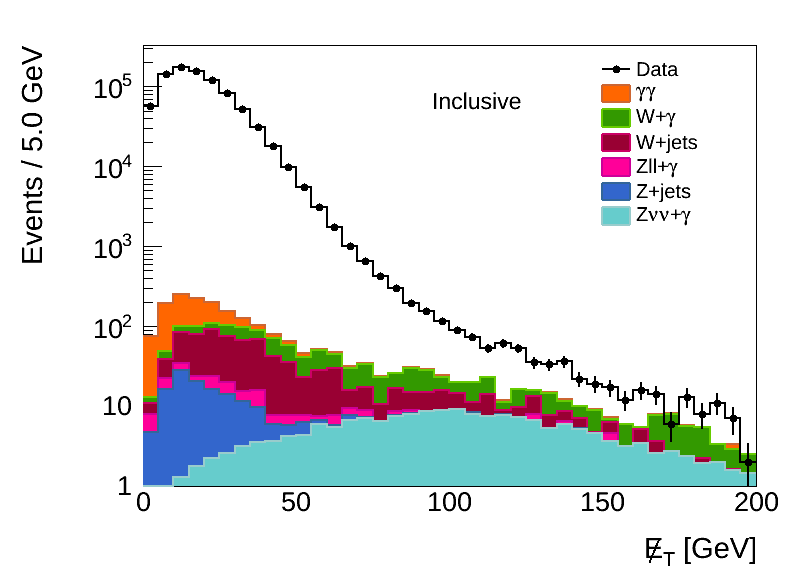
\includegraphics[width=.4\textwidth]{figures/rawmet1_incl_55up.png}}
\subfigure[0-Jet]{\label{subfig:rawmet55up_0j}
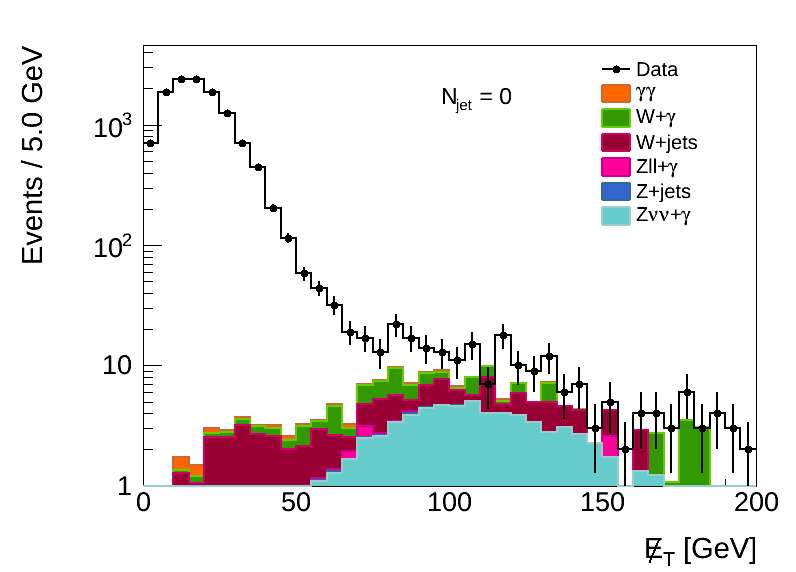
\includegraphics[width=.4\textwidth]{figures/rawmet1_0j_55up.png}} \\
\subfigure[1-Jet]{\label{subfig:rawmet55up_1j}
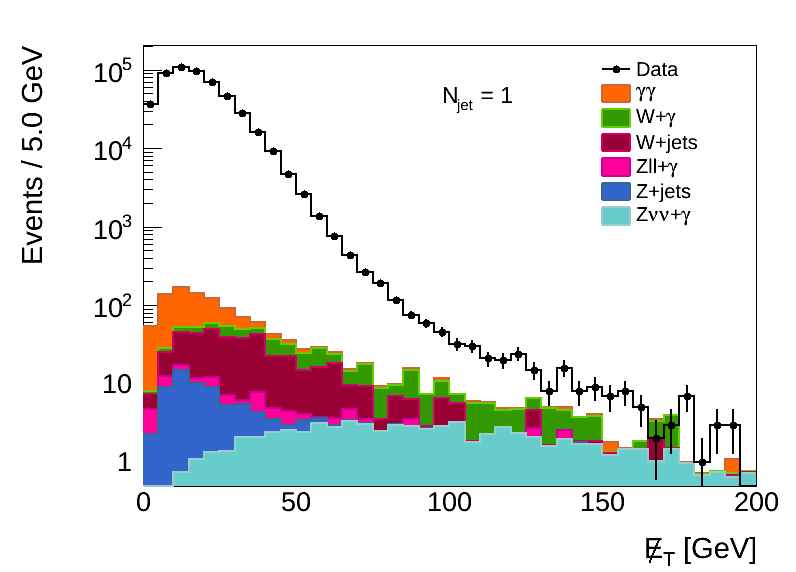
\includegraphics[width=.4\textwidth]{figures/rawmet1_1j_55up.png}}
\subfigure[$\geq$2 Jets]{\label{subfig:rawmet55up_2j}
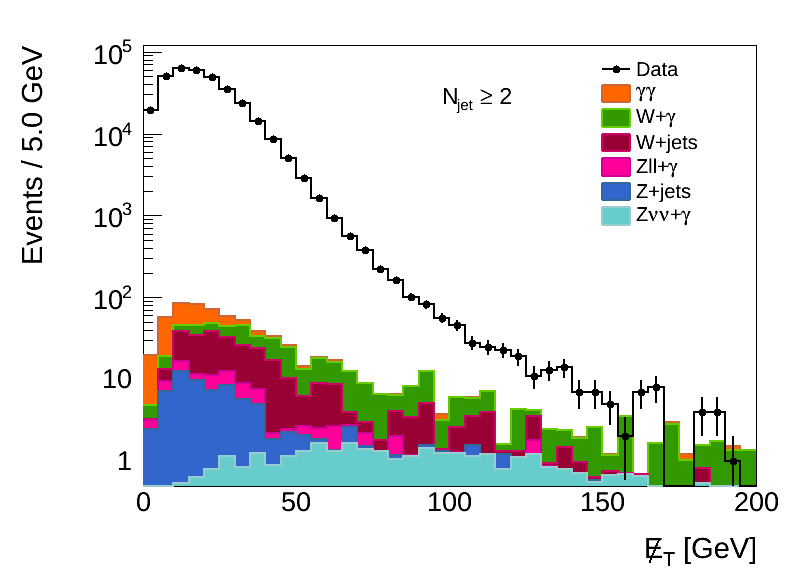
\includegraphics[width=.4\textwidth]{figures/rawmet1_2j_55up.png}}
\caption{MET distributions at the photon selection level for photons with $p_T>55\:\GeVc$ in the Inclusive~\subref{subfig:rawmet55up_incl}, 
0-Jet~\subref{subfig:rawmet55up_0j}, 1-Jet~\subref{subfig:rawmet55up_1j} and $\geq$2-Jets~\subref{subfig:rawmet55up_2j} bins, compared to 
the expected from simulation for signal and background. The MC contributions are stacked togther and overlaid on top of the data histogram.}
\label{fig:rawmet55up}
\end{center}
\end{figure}
%%%%%%%%

%%%%%%%%
\begin{figure}[!hbtp]
\begin{center}
\subfigure[Inclusive]{\label{subfig:rawmet55to80_incl}
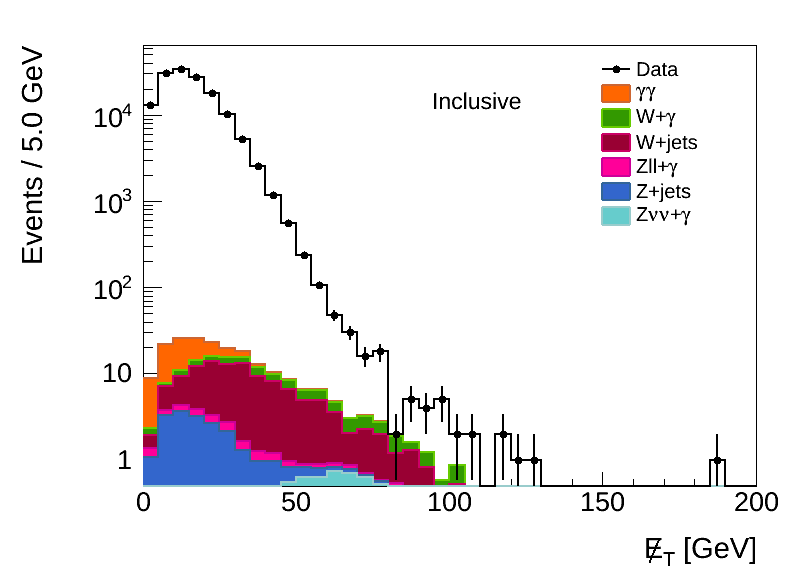
\includegraphics[width=.4\textwidth]{figures/rawmet1_incl_55to80.png}}
\subfigure[0-Jet]{\label{subfig:rawmet55to80_0j}
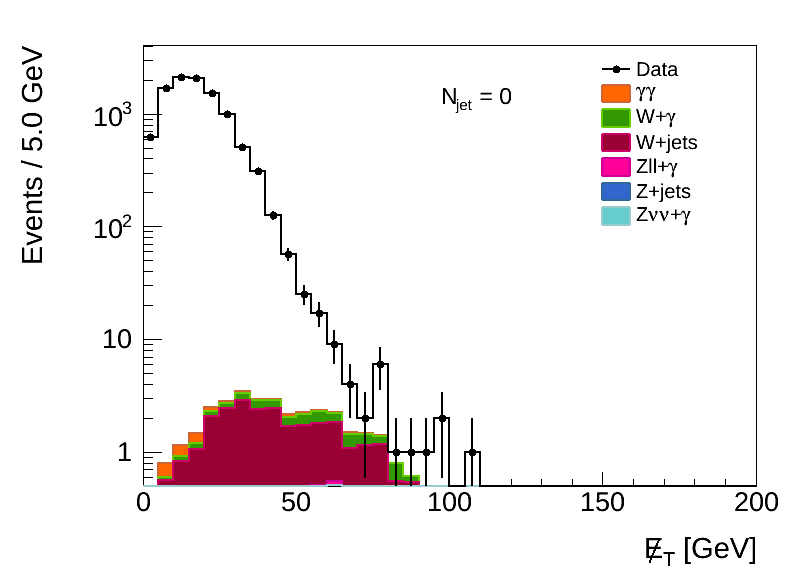
\includegraphics[width=.4\textwidth]{figures/rawmet1_0j_55to80.png}} \\
\subfigure[1-Jet]{\label{subfig:rawmet55to80_1j}
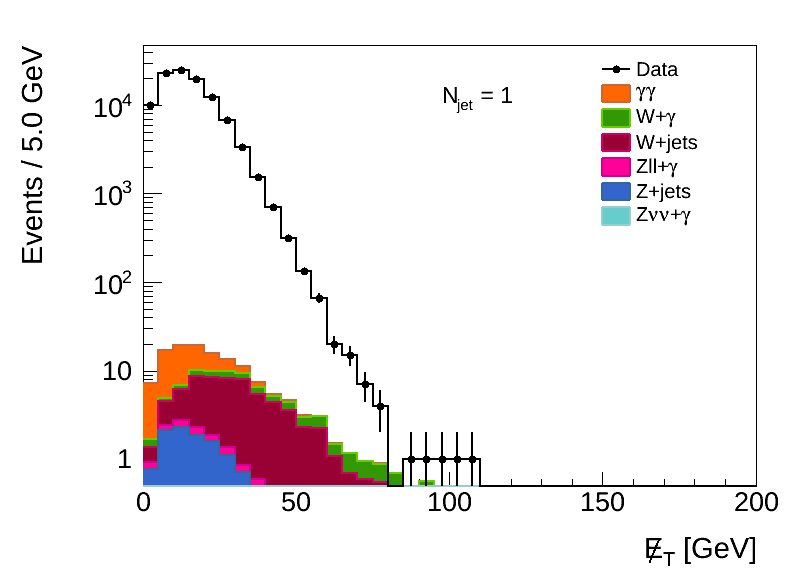
\includegraphics[width=.4\textwidth]{figures/rawmet1_1j_55to80.png}}
\subfigure[$\geq$2 Jets]{\label{subfig:rawmet55to80_2j}
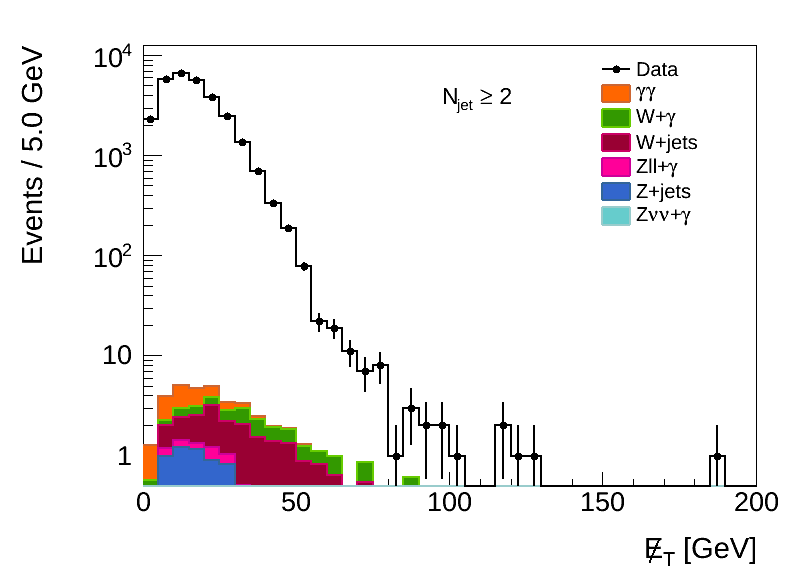
\includegraphics[width=.4\textwidth]{figures/rawmet1_2j_55to80.png}}
\caption{MET distributions at the photon selection level for photons with $55\:\GeVc<p_T<80\:\GeVc$ in the Inclusive~\subref{subfig:rawmet55to80_incl}, 
0-Jet~\subref{subfig:rawmet55to80_0j}, 1-Jet~\subref{subfig:rawmet55to80_1j} and $\geq$2-Jets~\subref{subfig:rawmet55to80_2j} bins, compared to 
the expected from simulation for signal and background. The MC contributions are stacked togther and overlaid on top of the data histogram.}
\label{fig:rawmet55to80}
\end{center}
\end{figure}
%%%%%%%%

%%%%%%%%
\begin{figure}[!hbtp]
\begin{center}
\subfigure[Inclusive]{\label{subfig:rawmet80to95_incl}
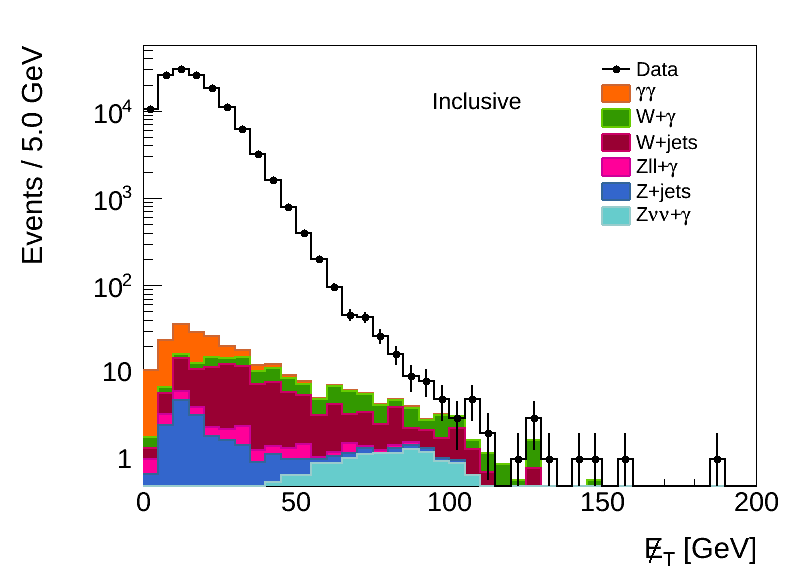
\includegraphics[width=.4\textwidth]{figures/rawmet1_incl_80to95.png}}
\subfigure[0-Jet]{\label{subfig:rawmet80to95_0j}
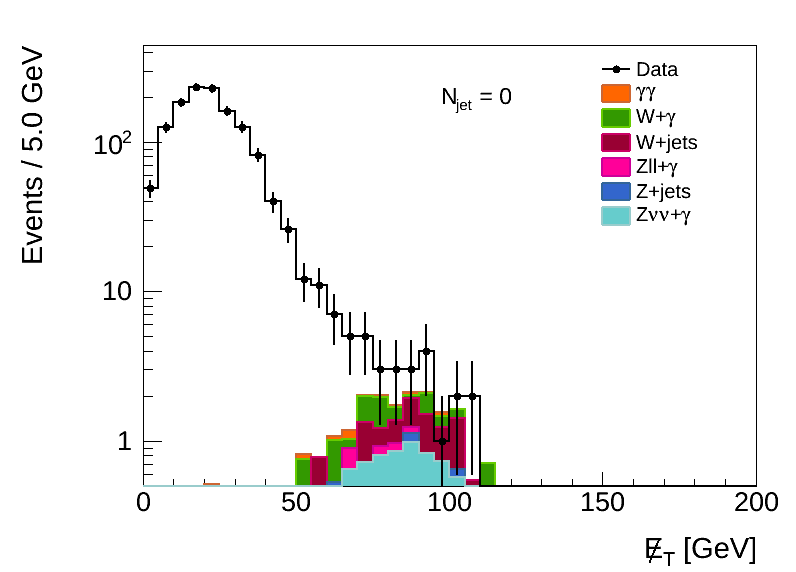
\includegraphics[width=.4\textwidth]{figures/rawmet1_0j_80to95.png}} \\
\subfigure[1-Jet]{\label{subfig:rawmet80to95_1j}
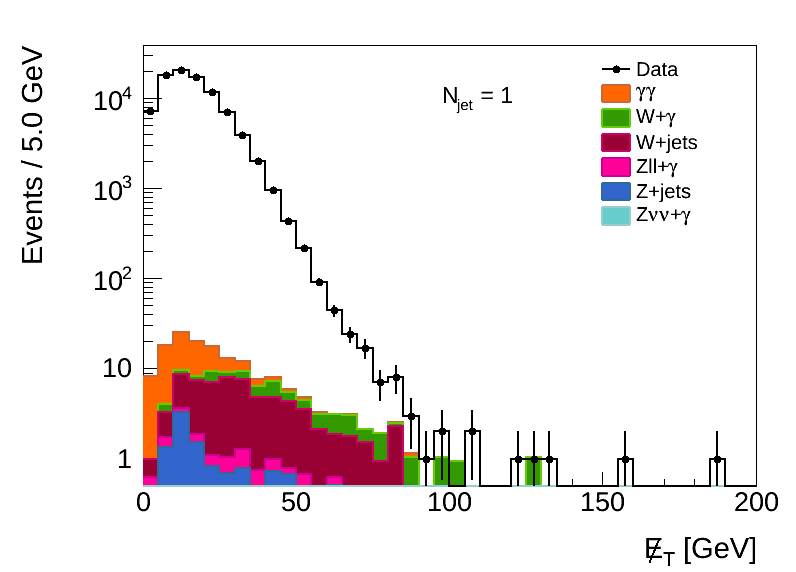
\includegraphics[width=.4\textwidth]{figures/rawmet1_1j_80to95.png}}
\subfigure[$\geq$2 Jets]{\label{subfig:rawmet80to95_2j}
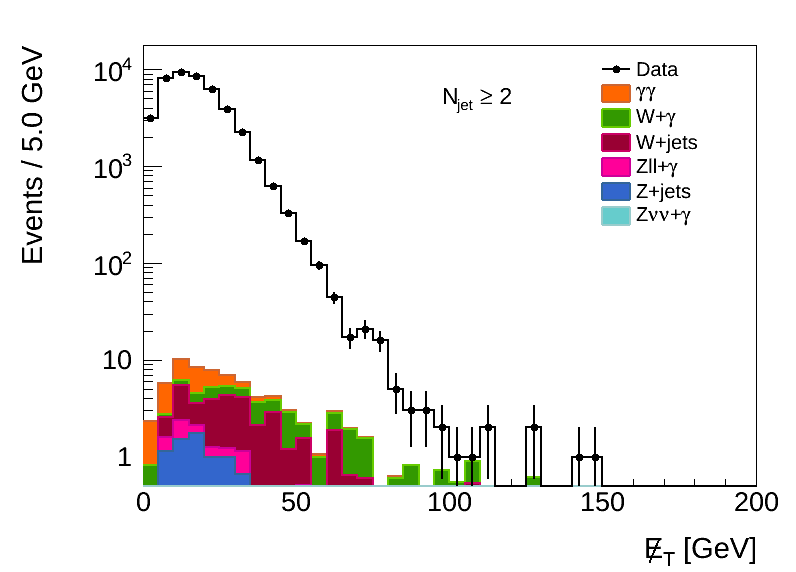
\includegraphics[width=.4\textwidth]{figures/rawmet1_2j_80to95.png}}
\caption{MET distributions at the photon selection level for photons with $80\:\GeVc<p_T<95\:\GeVc$ in the Inclusive~\subref{subfig:rawmet80to95_incl}, 
0-Jet~\subref{subfig:rawmet80to95_0j}, 1-Jet~\subref{subfig:rawmet80to95_1j} and $\geq$2-Jets~\subref{subfig:rawmet80to95_2j} bins, compared to 
the expected from simulation for signal and background. The MC contributions are stacked togther and overlaid on top of the data histogram.}
\label{fig:rawmet80to95}
\end{center}
\end{figure}
%%%%%%%%

%%%%%%%%
\begin{figure}[!hbtp]
\begin{center}
\subfigure[Inclusive]{\label{subfig:rawmet95up_incl}
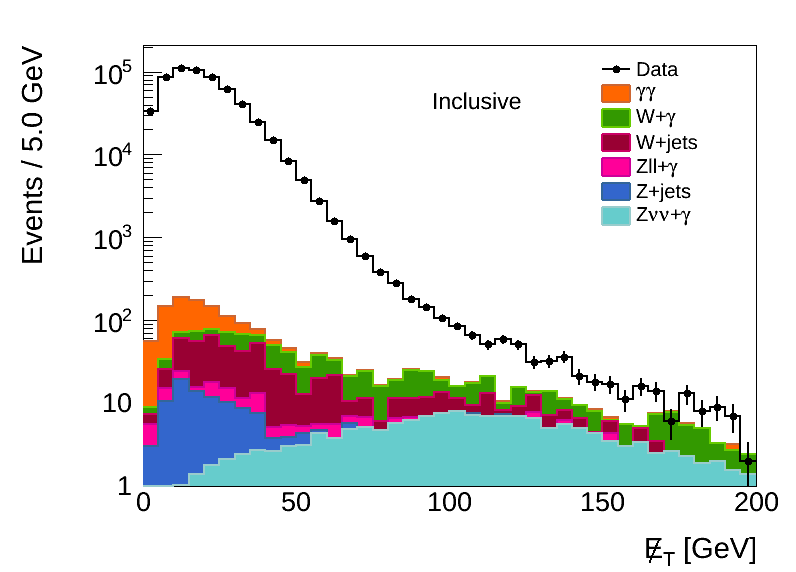
\includegraphics[width=.4\textwidth]{figures/rawmet1_incl_95up.png}}
\subfigure[0-Jet]{\label{subfig:rawmet95up_0j}
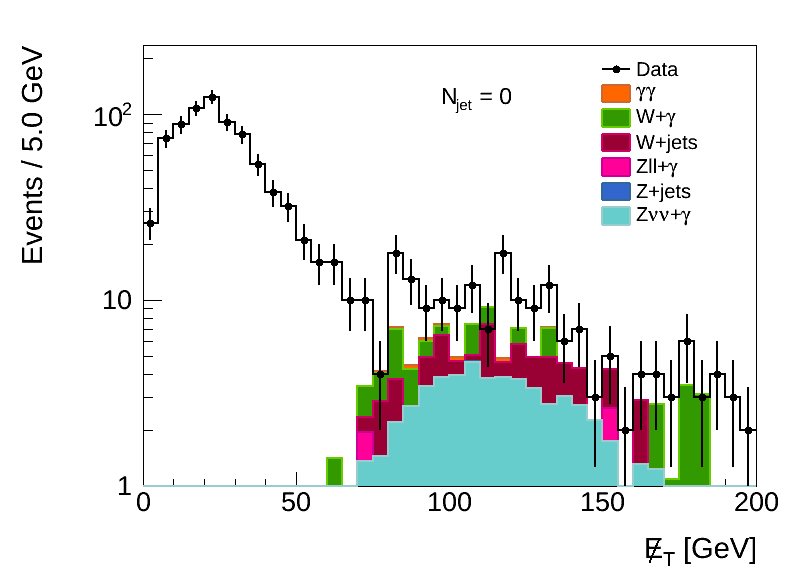
\includegraphics[width=.4\textwidth]{figures/rawmet1_0j_95up.png}} \\
\subfigure[1-Jet]{\label{subfig:rawmet95up_1j}
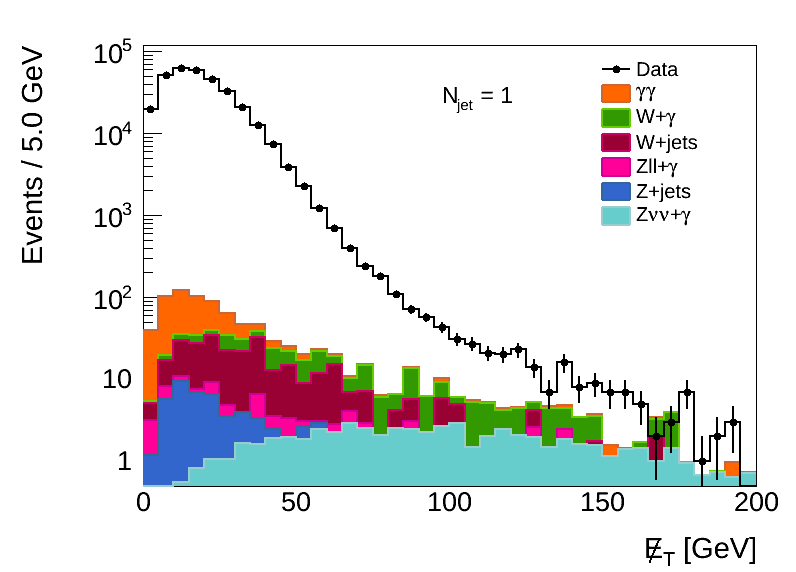
\includegraphics[width=.4\textwidth]{figures/rawmet1_1j_95up.png}}
\subfigure[$\geq$2 Jets]{\label{subfig:rawmet95up_2j}
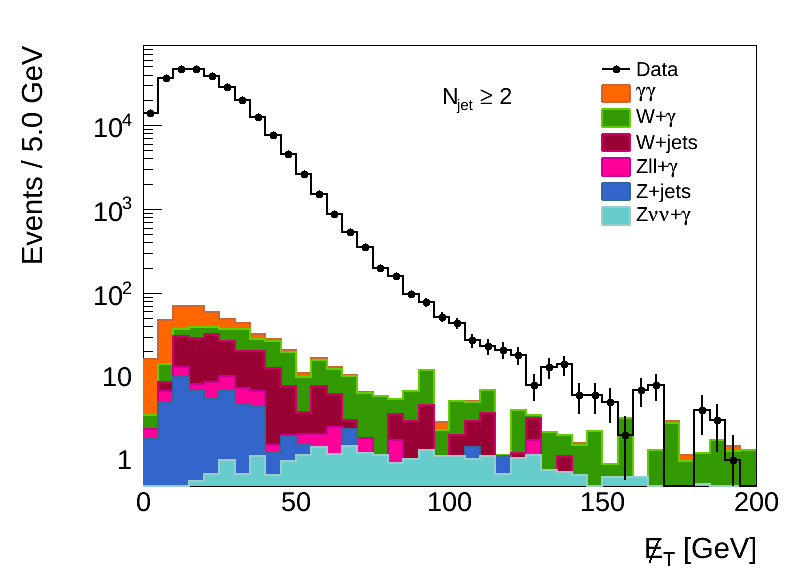
\includegraphics[width=.4\textwidth]{figures/rawmet1_2j_95up.png}}
\caption{MET distributions at the photon selection level for photons with $p_T>95\:\GeVc$ in the Inclusive~\subref{subfig:rawmet95up_incl}, 
0-Jet~\subref{subfig:rawmet95up_0j}, 1-Jet~\subref{subfig:rawmet95up_1j} and $\geq$2-Jets~\subref{subfig:rawmet95up_2j} bins, compared to 
the expected from simulation for signal and background. The MC contributions are stacked togther and overlaid on top of the data histogram.}
\label{fig:rawmet95up}
\end{center}
\end{figure}
%%%%%%%%

\clearpage

The contamination after re-weighting the photon events to give a prediction for $Z(\mu\mu)+$jets is summarized in Table~\ref{tab:rawyieldsmm}.
Since the photon $p_T$ spectrum is softer for $W$ events compared to $Z(\nu\nu)+\gamma$, the relative contributions from $W+\gamma$ and $W+$jets
are increased after re-weighting since the weights are higher at lower $p_T$. The plots of the MET distributions are shown in 
Figs.~\ref{fig:weightedmet55up} -~\ref{fig:weightedmet95up}.

\begin{table}[!ht]
\begin{center}
{\footnotesize
\begin{tabular}{c|c|c|c}
\hline
 &  0-jet  &  1-jet  &  2+ jets  \\
\hline\hline
$\gamma+$jets data            & $64.05 \pm 7.10$  &  $506.31 \pm 16.23$  &  $437.53 \pm 10.84$ \\
\hline
$Z(\nu\nu)+\gamma$            & $4.40 \pm 0.06$   &  $3.70 \pm 0.06$	 &  $1.64 \pm 0.04$ \\
$W+$jets                      & $3.80 \pm 0.31$   &  $5.87 \pm 0.44$	 &  $2.91 \pm 0.29$ \\
$W+\gamma$                    & $2.35 \pm 0.24$   &  $6.05 \pm 0.44$	 &  $4.99 \pm 0.40$ \\
$Z+$jets                      & $0.08 \pm 0.02$   &  $0.22 \pm 0.04$	 &  $0.27 \pm 0.05$ \\
$Z(\ell\ell)+\gamma$          & $0.17 \pm 0.05$   &  $0.32 \pm 0.08$	 &  $0.29 \pm 0.07$ \\
$\gamma\gamma$                & $0.22 \pm 0.02$   &  $9.59 \pm 0.06$	 &  $0.23 \pm 0.03$ \\
\hline
Bkg. Sub. $\gamma+$jets data  & $53.04 \pm 7.11$  &  $489.57 \pm 16.24$  &  $427.79 \pm 10.85$ \\
\hline
Purity [\%]                   & $83 \pm 9$        &  $97 \pm 3$          &  $98 \pm 2$ \\
\hline
\end{tabular}
}
\caption{Z+jets prediction in the dimuon channel for MET$>50\:\GeV$.}
\label{tab:weightedyieldsmm}
\end{center}
\end{table}

%%%%%%%%
\begin{figure}[!hbtp]
\begin{center}
\subfigure[Inclusive]{\label{subfig:weightedmet55up_incl}
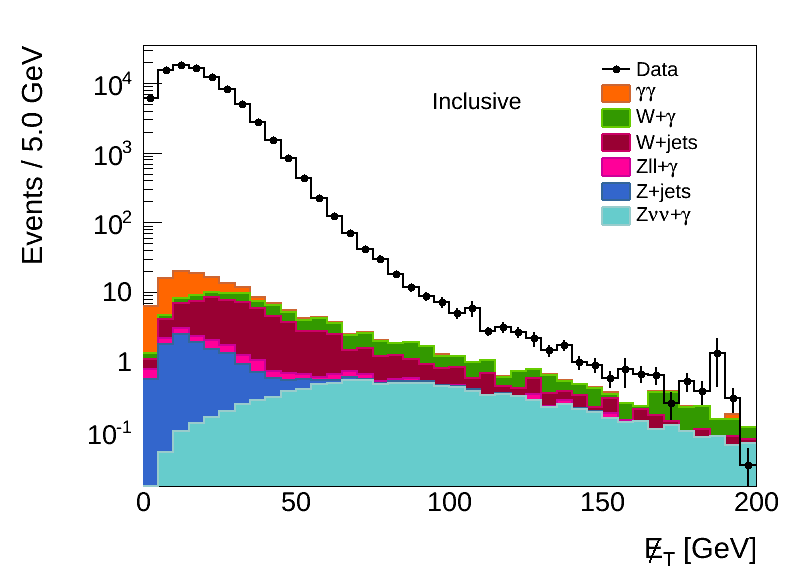
\includegraphics[width=.4\textwidth]{figures/weightedmet1_incl_55up.png}}
\subfigure[0-Jet]{\label{subfig:weightedmet55up_0j}
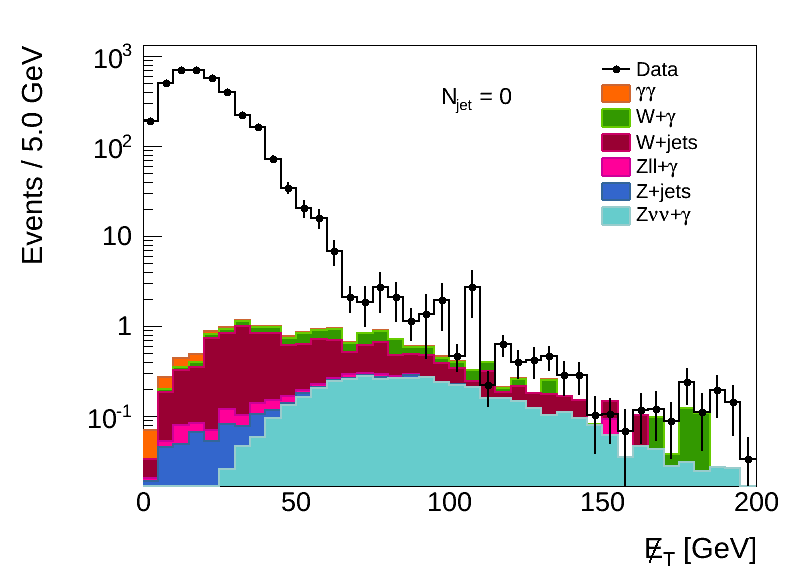
\includegraphics[width=.4\textwidth]{figures/weightedmet1_0j_55up.png}} \\
\subfigure[1-Jet]{\label{subfig:weightedmet55up_1j}
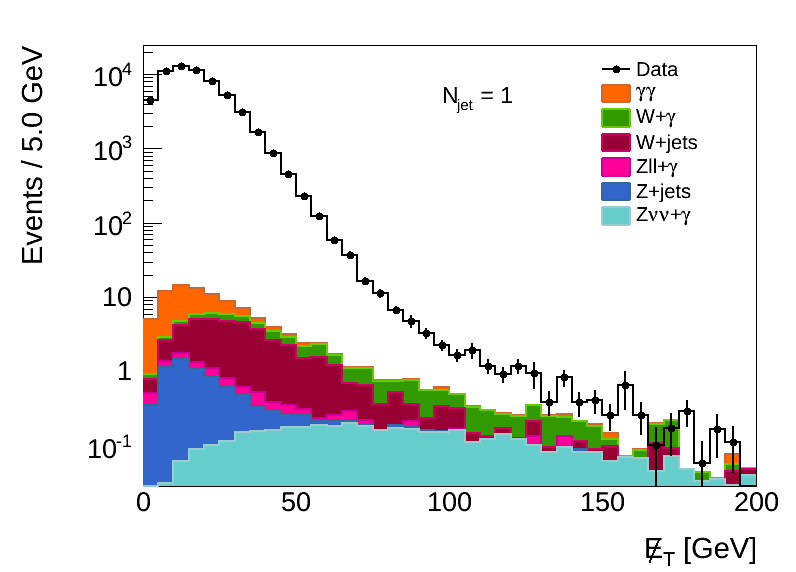
\includegraphics[width=.4\textwidth]{figures/weightedmet1_1j_55up.png}}
\subfigure[$\geq$2 Jets]{\label{subfig:weightedmet55up_2j}
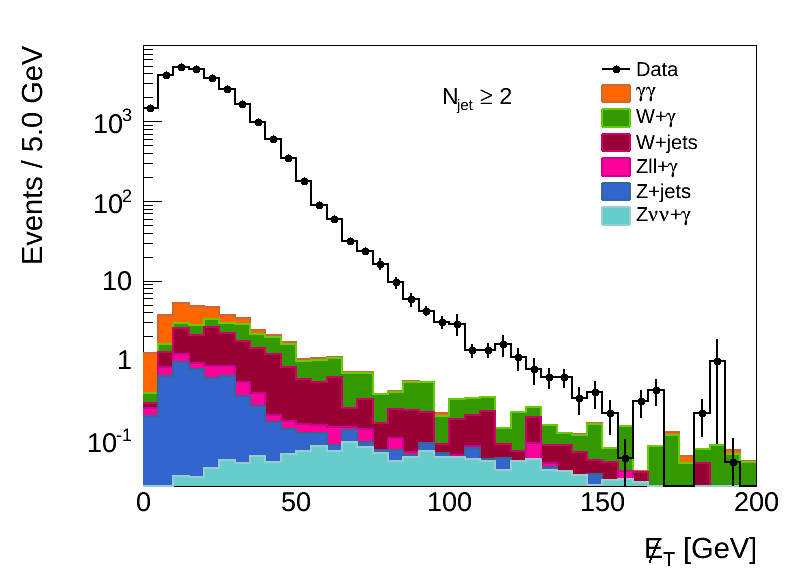
\includegraphics[width=.4\textwidth]{figures/weightedmet1_2j_55up.png}}
\caption{MET distributions after re-weighting to dimuons for photons with $p_T>55\:\GeVc$ in the Inclusive~\subref{subfig:weightedmet55up_incl}, 
0-Jet~\subref{subfig:weightedmet55up_0j}, 1-Jet~\subref{subfig:weightedmet55up_1j} and $\geq$2-Jets~\subref{subfig:weightedmet55up_2j} bins, 
compared to the expected from simulation for signal and background. The MC contributions are stacked togther and overlaid on top of the data 
histogram.}
\label{fig:weightedmet55up}
\end{center}
\end{figure}
%%%%%%%%

%%%%%%%%
\begin{figure}[!hbtp]
\begin{center}
\subfigure[Inclusive]{\label{subfig:weightedmet55to80_incl}
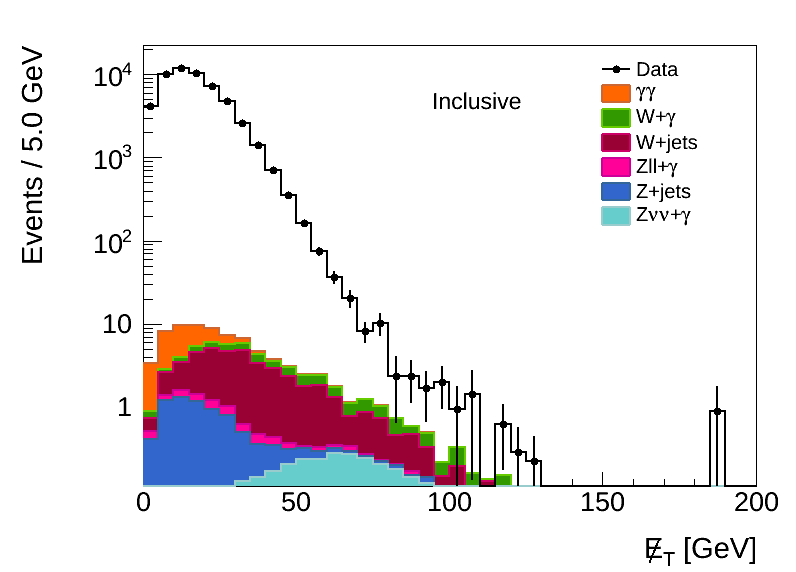
\includegraphics[width=.4\textwidth]{figures/weightedmet1_incl_55to80.png}}
\subfigure[0-Jet]{\label{subfig:weightedmet55to80_0j}
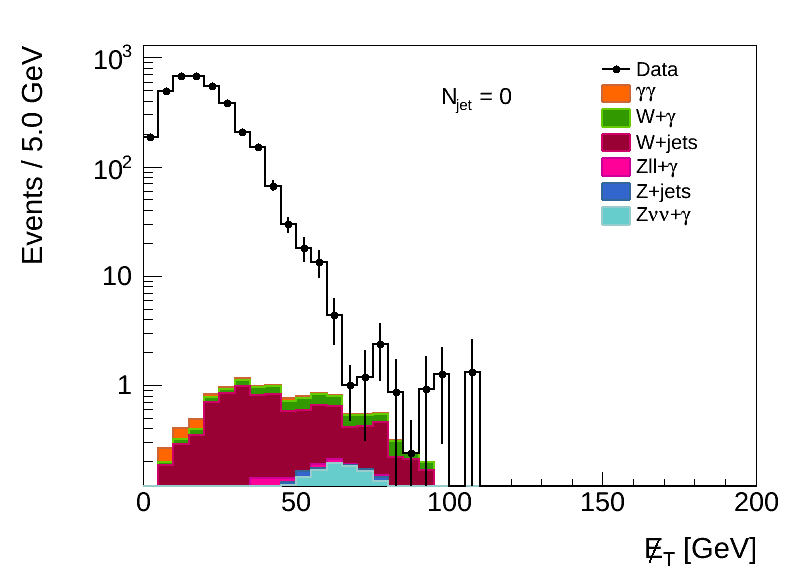
\includegraphics[width=.4\textwidth]{figures/weightedmet1_0j_55to80.png}} \\
\subfigure[1-Jet]{\label{subfig:weightedmet55to80_1j}
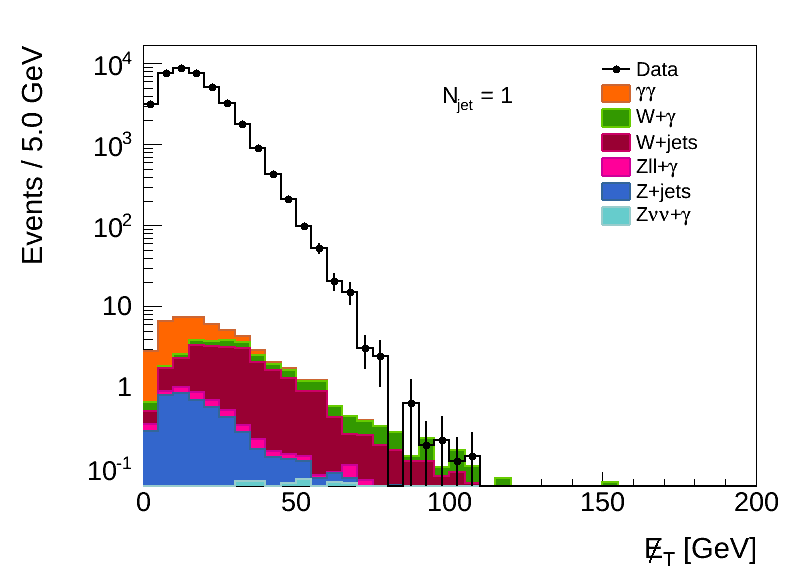
\includegraphics[width=.4\textwidth]{figures/weightedmet1_1j_55to80.png}}
\subfigure[$\geq$2 Jets]{\label{subfig:weightedmet55to80_2j}
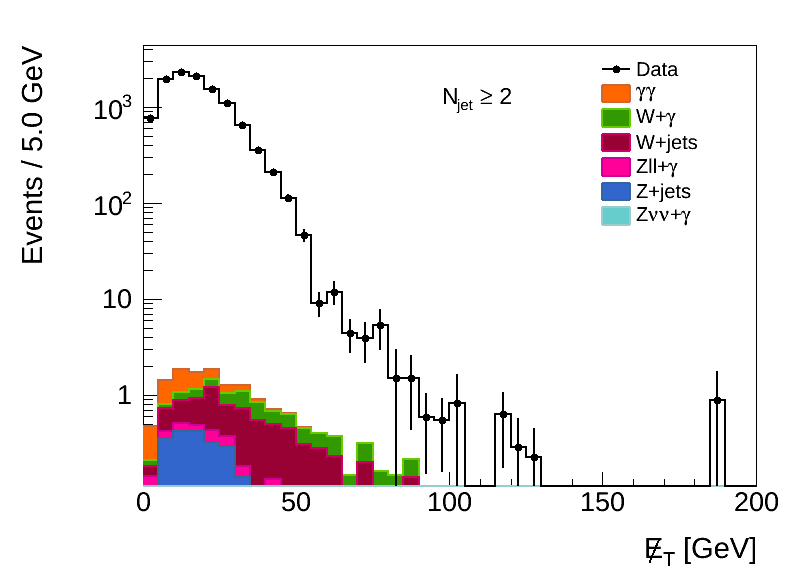
\includegraphics[width=.4\textwidth]{figures/weightedmet1_2j_55to80.png}}
\caption{MET distributions after re-weighting to dimuons for photons with $55\:\GeVc<p_T<80\:\GeVc$ in the Inclusive~\subref{subfig:weightedmet55to80_incl}, 
0-Jet~\subref{subfig:weightedmet55to80_0j}, 1-Jet~\subref{subfig:weightedmet55to80_1j} and $\geq$2-Jets~\subref{subfig:weightedmet55to80_2j} bins, 
compared to the expected from simulation for signal and background. The MC contributions are stacked togther and overlaid on top of the data 
histogram.}
\label{fig:weightedmet55to80}
\end{center}
\end{figure}
%%%%%%%%

%%%%%%%%
\begin{figure}[!hbtp]
\begin{center}
\subfigure[Inclusive]{\label{subfig:weightedmet80to95_incl}
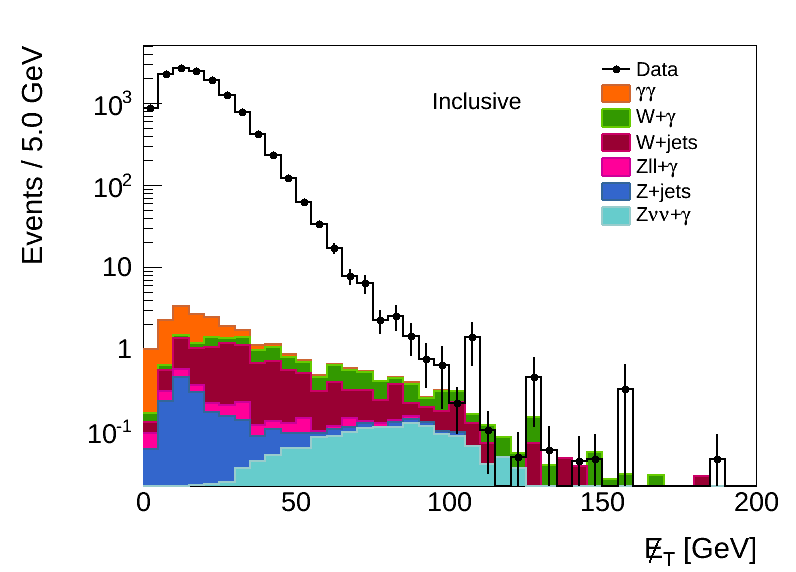
\includegraphics[width=.4\textwidth]{figures/weightedmet1_incl_80to95.png}}
\subfigure[0-Jet]{\label{subfig:weightedmet80to95_0j}
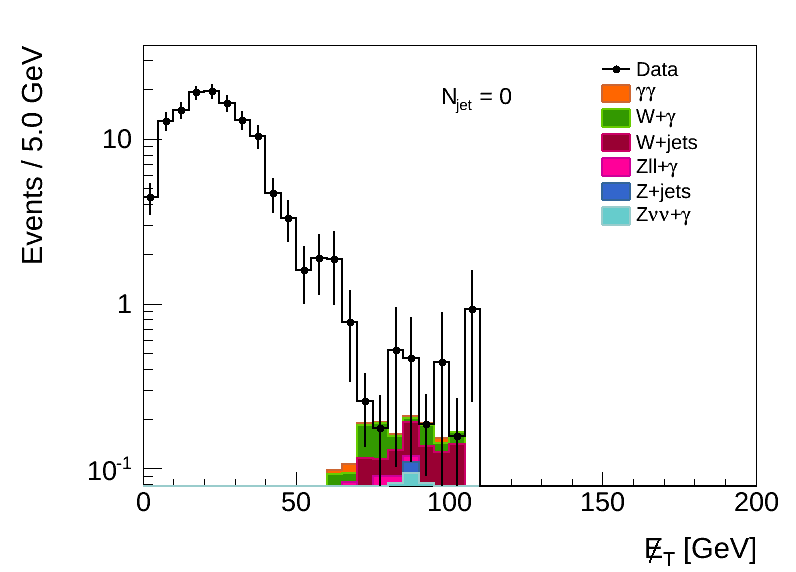
\includegraphics[width=.4\textwidth]{figures/weightedmet1_0j_80to95.png}} \\
\subfigure[1-Jet]{\label{subfig:weightedmet80to95_1j}
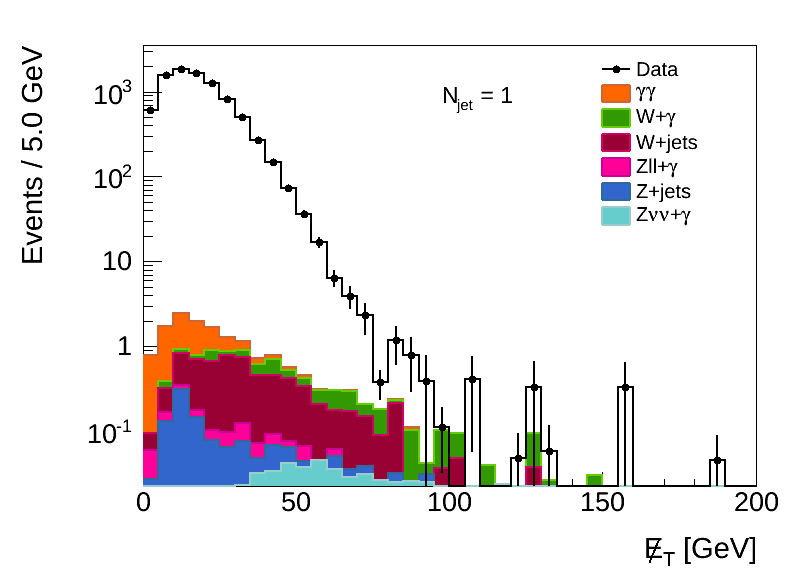
\includegraphics[width=.4\textwidth]{figures/weightedmet1_1j_80to95.png}}
\subfigure[$\geq$2 Jets]{\label{subfig:weightedmet80to95_2j}
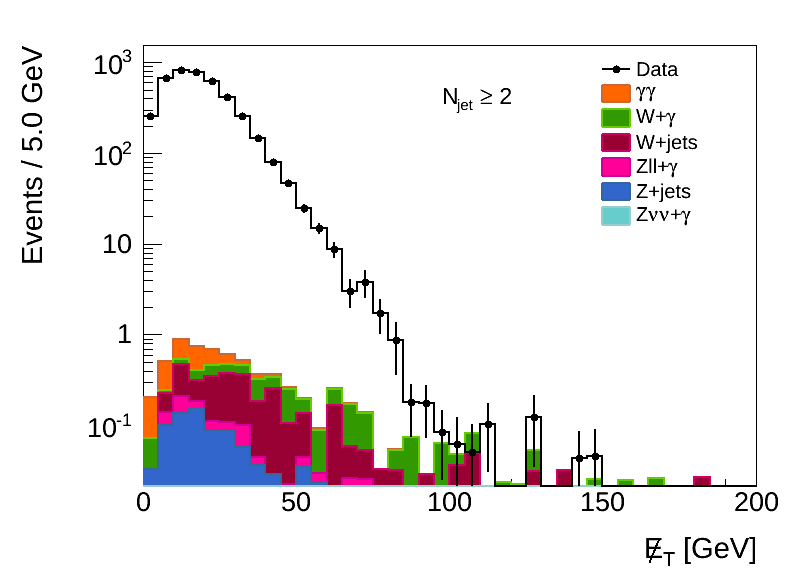
\includegraphics[width=.4\textwidth]{figures/weightedmet1_2j_80to95.png}}
\caption{MET distributions after re-weighting to dimuons for photons with $80\:\GeVc<p_T<95\:\GeVc$ in the Inclusive~\subref{subfig:weightedmet80to95_incl}, 
0-Jet~\subref{subfig:weightedmet80to95_0j}, 1-Jet~\subref{subfig:weightedmet80to95_1j} and $\geq$2-Jets~\subref{subfig:weightedmet80to95_2j} bins, 
compared to the expected from simulation for signal and background. The MC contributions are stacked togther and overlaid on top of the data 
histogram.}
\label{fig:weightedmet80to95}
\end{center}
\end{figure}
%%%%%%%%

%%%%%%%%
\begin{figure}[!hbtp]
\begin{center}
\subfigure[Inclusive]{\label{subfig:weightedmet95up_incl}
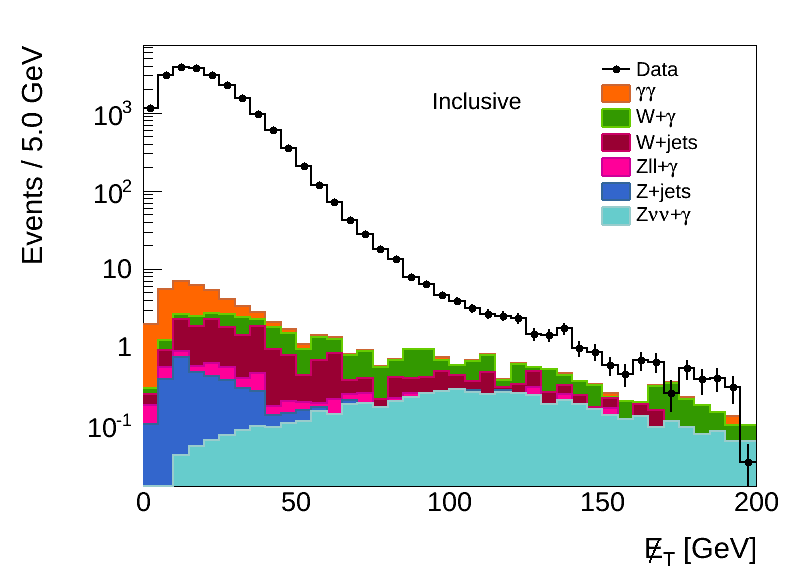
\includegraphics[width=.4\textwidth]{figures/weightedmet1_incl_95up.png}}
\subfigure[0-Jet]{\label{subfig:weightedmet95up_0j}
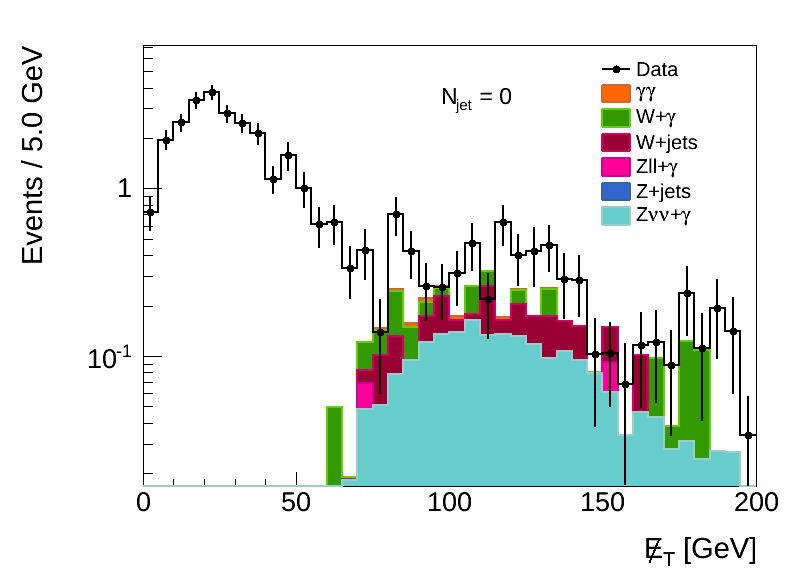
\includegraphics[width=.4\textwidth]{figures/weightedmet1_0j_95up.png}} \\
\subfigure[1-Jet]{\label{subfig:weightedmet95up_1j}
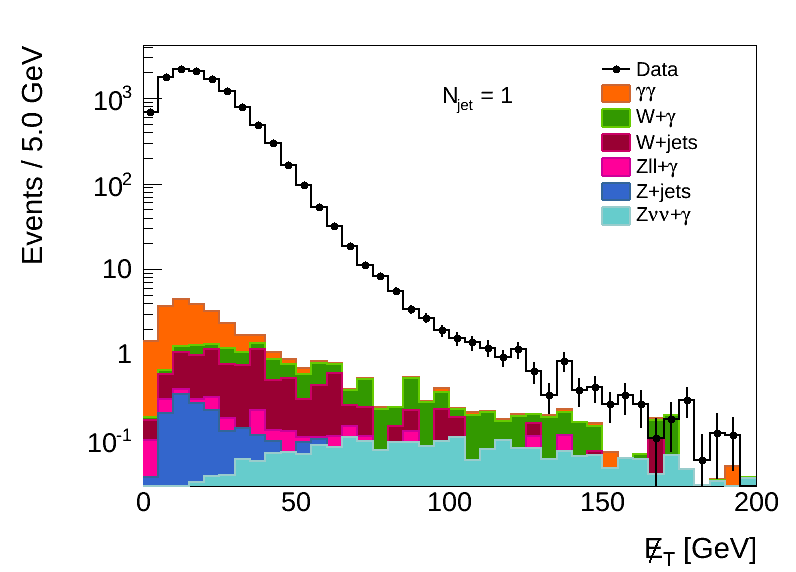
\includegraphics[width=.4\textwidth]{figures/weightedmet1_1j_95up.png}}
\subfigure[$\geq$2 Jets]{\label{subfig:weightedmet95up_2j}
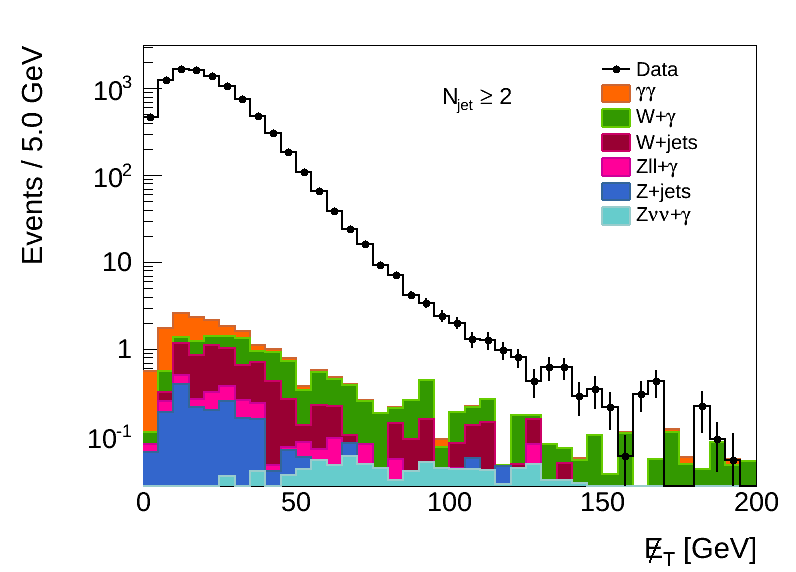
\includegraphics[width=.4\textwidth]{figures/weightedmet1_2j_95up.png}}
\caption{MET distributions after re-weighting to dimuons for photons with $p_T>95\:\GeVc$ in the Inclusive~\subref{subfig:weightedmet95up_incl}, 
0-Jet~\subref{subfig:weightedmet95up_0j}, 1-Jet~\subref{subfig:weightedmet95up_1j} and $\geq$2-Jets~\subref{subfig:weightedmet95up_2j} bins, 
compared to the expected from simulation for signal and background. The MC contributions are stacked togther and overlaid on top of the data 
histogram.}
\label{fig:weightedmet95up}
\end{center}
\end{figure}
%%%%%%%%

\clearpage

The contamination after applying $m_H=250\:\GeVcc$ cut-based selection cuts to give a prediction for $Z(\mu\mu)+$jets is summarized in 
Table~\ref{tab:rawyieldsmm}. The purity of the $\gamma+$jets sample is between $50\%$ to $65\%$ depending on the jet multiplicity.
The plots of the MET distributions are shown in Fig.~\ref{fig:selectmet55up}.

\begin{table}[!ht]
\begin{center}
{\footnotesize
\begin{tabular}{c|c|c|c}
\hline
 &  0-jet  &  1-jet  &  2+ jets  \\
\hline\hline
$\gamma+$jets data            & $8.64 \pm 2.43$   &  $6.22 \pm 1.30$   &  $3.98 \pm 0.72$ \\
\hline
$Z(\nu\nu)+\gamma$            & $1.28 \pm 0.03$   &  $0.90  \pm 0.02$  &  $0.28  \pm 0.01$ \\
$W+$jets                      & $1.03 \pm 0.14$   &  $0.63  \pm 0.13$  &  $0.20  \pm 0.08$ \\
$W+\gamma$                    & $0.64 \pm 0.12$   &  $1.17  \pm 0.18$  &  $0.74  \pm 0.14$ \\
$Z+$jets                      & $0.01 \pm 0.01$   &  $0.005 \pm 0.004$ &  $0.004 \pm 0.004$ \\
$Z(\ell\ell)+\gamma$          & $0.03 \pm 0.02$   &  $0.02  \pm 0.01$  &  $0.02  \pm 0.01$ \\
$\gamma\gamma$                & $0.04 \pm 0.01$   &  $0.03  \pm 0.01$  &  $0.003 \pm 0.002$ \\
\hline
Bkg. Sub. $\gamma+$jets data  & $5.56 \pm 2.44$   &  $3.48  \pm 1.32$  &  $2.74  \pm 0.73$ \\
\hline
Purity [\%]                   & $65 \pm 18$       &  $51 \pm 13$       &  $62 \pm 13$ \\
\hline
\end{tabular}
}
\caption{Z+jets prediction in the dimuon channel for the $m_H = 250\:\GeVcc$ selection.}
\label{tab:mh250yieldsmm}
\end{center}
\end{table}

%%%%%%%%
\begin{figure}[!hbtp]
\begin{center}
\subfigure[Inclusive]{\label{subfig:selectmet55up_incl}
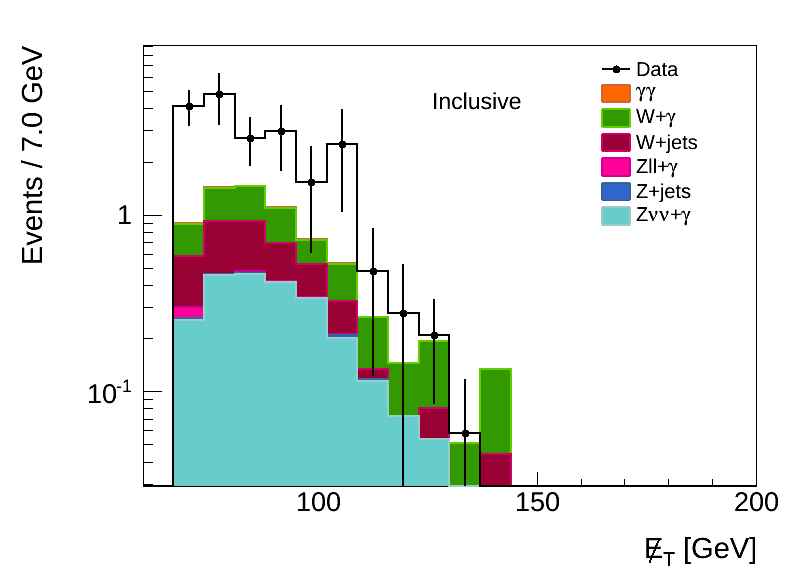
\includegraphics[width=.4\textwidth]{figures/selectmet_incl_55up.png}}
\subfigure[0-Jet]{\label{subfig:selectmet55up_0j}
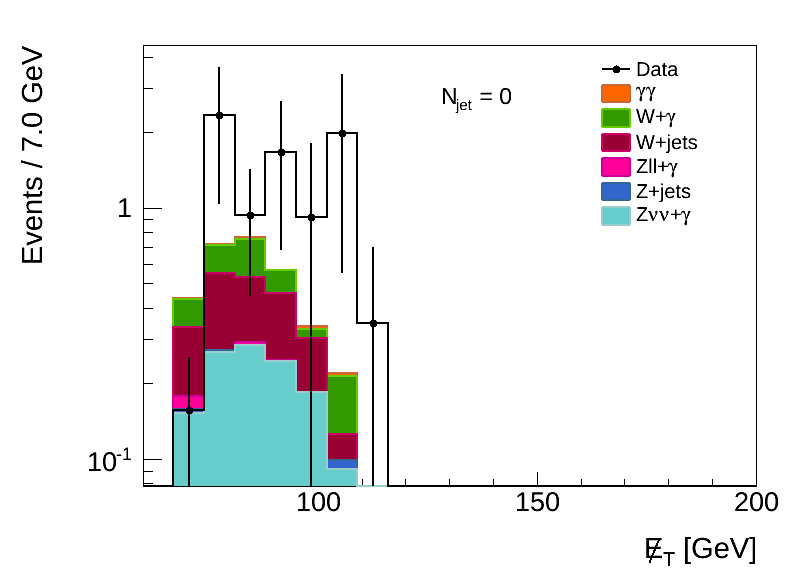
\includegraphics[width=.4\textwidth]{figures/selectmet_0j_55up.png}} \\
\subfigure[1-Jet]{\label{subfig:selectmet55up_1j}
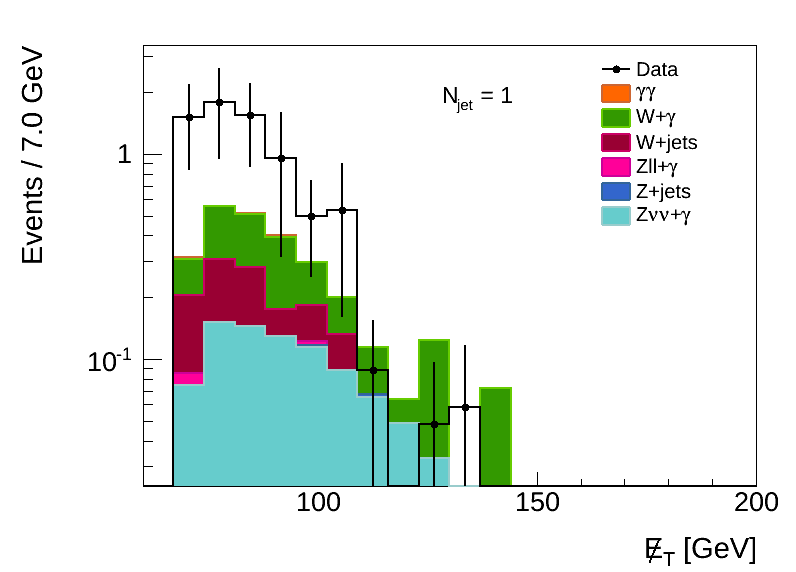
\includegraphics[width=.4\textwidth]{figures/selectmet_1j_55up.png}}
\subfigure[$\geq$2 Jets]{\label{subfig:selectmet55up_2j}
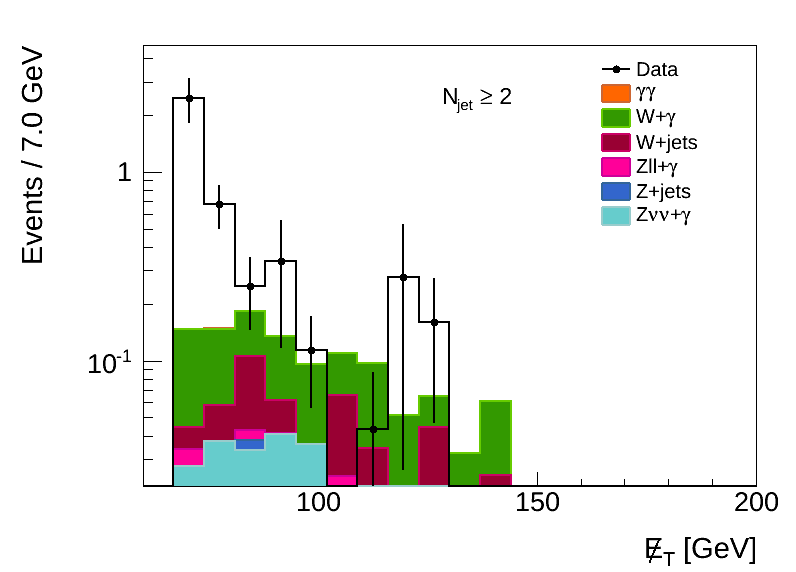
\includegraphics[width=.4\textwidth]{figures/selectmet_2j_55up.png}}
\caption{MET distributions after $m_H=250\:\GeVcc$ cut-based selection in the Inclusive~\subref{subfig:selectmet55up_incl}, 
0-Jet~\subref{subfig:selectmet55up_0j}, 1-Jet~\subref{subfig:selectmet55up_1j} and $\geq$2-Jets~\subref{subfig:selectmet55up_2j} bins, 
compared to the expected from simulation for signal and background. The MC contributions are stacked togther and overlaid on 
top of the data histogram.}
\label{fig:selectmet55up}
\end{center}
\end{figure}
%%%%%%%%

\clearpage

The $Z$+jets predictions for various $m_H$ selection cuts are listed in Table~\ref{tab:corrpredict} before and after subtracting for
contamination. The predictions are for the combined dielectron and dimuon channels. Recall that the current prescription is to claim
the uncorrected prediction as the upper bound then taking the central value as half of the upper bound and quoting $100\%$ uncertainty.  

\begin{table}[!ht]
\begin{center}
{\footnotesize
\begin{tabular}{|c|c|c|c|}
\hline
  $m_H [\GeVcc]$ &  Uncorrected  &  Corrected \\
\hline
$250$  & $32.84 \pm 3.54$   &  $21.07 \pm 0.40$ \\
$300$  & $14.73 \pm 1.15$   &  $5.86  \pm 0.44$ \\
$350$  & $9.08  \pm 0.61$   &  $3.53  \pm 0.35$ \\
$400$  & $5.03  \pm 0.45$   &  $1.05  \pm 0.29$ \\
$500$  & $2.70  \pm 0.33$   &  $0.87  \pm 0.16$ \\
$600$  & $1.27  \pm 0.23$   &  $0.44  \pm 0.10$ \\
\hline
\end{tabular}
}
\caption{Z+jets prediction for $ee$ and $\mu\mu$ combined for different $m_H$ hypotheses.}
\label{tab:corrpredict}
\end{center}
\end{table}
